%%%%%%%%%%%%%%%%%%%%%%%%%%%%%%%%%%%%%%%%
\section{Sampling Dist.\ of $(\bar{X} - \bar{Y})$ -- Normal Populations, Variances Known}
%%%%%%%%%%%%%%%%%%%%%%%%%%%%%%%%%%%%%%%%
\begin{frame}
\frametitle{Sampling Dist.\ of $(\bar{X}_n - \bar{Y}_m)$ -- Normal Popns.\ Vars.\ Known}

\small

Suppose $X_1, \hdots, X_{n} \sim \mbox{iid } N(\mu_x, \sigma^2_x)$ indep.\ of $Y_1, \hdots, Y_{m} \sim \mbox{iid } N(\mu_y, \sigma^2_y)$

\[SE(\bar{X}_n - \bar{Y}_m) = \sqrt{\displaystyle\frac{\sigma_x^2}{n} + \frac{\sigma_y^2}{m}}\]

\[\frac{\left(\bar{X}_n - \bar{Y}_m\right) - (\mu_x - \mu_y)}{SE(\bar{X}_n - \bar{Y}_m) } \sim N(0,1)\]

\vspace{1em}

\alert{You should be able to prove this using what we've learned about RVs.}



\end{frame}
%%%%%%%%%%%%%%%%%%%%%%%%%%%%%%%%%%%%%%%%
\begin{frame}
  \frametitle{CI for $(\mu_X - \mu_Y)$ -- Indep.\ Normal Popns.\, $\sigma_X^2, \sigma_Y^2$ Known}

	$$\alert{(\bar{X}_n - \bar{Y}_m) \pm \; \texttt{qnorm}(1-\alpha/2) \; SE(\bar{X}_n - \bar{Y}_m)}$$

  $$SE(\bar{X}_n - \bar{Y}_m) = \sqrt{\displaystyle\frac{\sigma_x^2}{n} + \frac{\sigma_y^2}{m} }$$
\end{frame}
%%%%%%%%%%%%%%%%%%%%%%%%%%%%%%%%%%%%%%%%
%\section{Sampling Dist.\ of $(\bar{X} - \bar{Y})$ -- Normal Popns, Variances Unknown}
%%%%%%%%%%%%%%%%%%%%%%%%%%%%%%%%%%%%%%%%%
%
%
%\begin{frame}
%\frametitle{What if $\sigma_x^2,\sigma_y^2$, are unknown?}
%
%$X_1, \hdots, X_{n} \sim \mbox{iid } N(\mu_x, \sigma^2_x)$ indep.\ of $Y_1, \hdots, Y_{m} \sim \mbox{iid } N(\mu_y, \sigma^2_y)$
%
%\[ \widehat{SE}(\bar{X}_n - \bar{Y}_m) = \sqrt{\displaystyle\frac{S_x^2}{n} + \frac{S_y^2}{m} }\]
%
%\[\frac{\left(\bar{X}_n - \bar{Y}_m\right) - (\mu_x - \mu_y)}{\widehat{SE}(\bar{X}_n - \bar{Y}_m)}\sim t(\nu)\]
%
%
%\begin{block}{Formula for $\nu$ is complicated and you don't need to know it}
%Two possibilities:
%	\begin{enumerate}
%		\item Have R find the correct value of $\nu$ for us
%		\item If $m,n$ are both large then so is $\nu$, hence $t(\nu) \approx N(0,1)$
%	\end{enumerate}
%\end{block}
%
%\end{frame}
%%%%%%%%%%%%%%%%%%%%%%%%%%%%%%%%%%%%%%%%%
%\section{Danger: Don't Assume Equal Variances Across Populations!}
%%%%%%%%%%%%%%%%%%%%%%%%%%%%%%%%%%%%%%%%%
%\begin{frame}
%\frametitle{Case of Equal, Unknown Variances}
%
%The book considers a case where $\sigma^2_x = \sigma^2_y = \sigma^2$, that is a common unknown variance. This is a \alert{very dangerous assumption}. It is almost certainly false and can throw off our results in a serious way. You are not responsible for this case.
%\end{frame}
%%%%%%%%%%%%%%%%%%%%%%%%%%%%%%%%%%%%%%%%
\section{CI for Difference of Population Means Using CLT}
%%%%%%%%%%%%%%%%%%%%%%%%%%%%%%%%%%%%%%%%
\begin{frame}
\frametitle{CI for Difference of Population Means Using CLT}
\begin{block}{Setup: Independent Random Samples}
$X_1, \hdots, X_n \sim \mbox{iid}$ with unknown mean $\mu_X$ \& unknown variance $\sigma_X^2$\\ $Y_1, \hdots, Y_m \sim \mbox{iid}$ with unknown mean $\mu_Y$ \& unknown variance $\sigma_Y^2$\\
\emph{where each sample is independent of the other } 
\end{block}

\begin{alertblock}{We Do Not Assume the Populations are Normal!}
\end{alertblock}

\end{frame}



%%%%%%%%%%%%%%%%%%%%%%%%%%%%%%%%%%%%%%%%
\begin{frame}
\frametitle{Difference of Sample Means $\bar{X}_n-\bar{Y}_m$ and the CLT}
\begin{block}{What We Have}
Approx.\ sampling dist.\ for \emph{individual}  sample means from CLT:
\[\alert{\bar{X}_n\approx N\left(\mu_X, S_X^2/n\right), \quad \bar{Y}_m\approx N\left(\mu_Y, S_Y^2/m\right)}\]
\end{block}

\begin{block}{What We Want}
Sampling Distribution of the \emph{difference} $\bar{X}_n - \bar{Y}_m$
\end{block}

\begin{block}{Use Independence of the Two Samples}
  
  \[\alert{\bar{X}_n - \bar{Y}_m\approx N\left( \mu_X - \mu_Y, \displaystyle \frac{S_X^2}{n} + \frac{S_Y^2}{m}\right)}\]

\end{block}


\end{frame}
%%%%%%%%%%%%%%%%%%%%%%%%%%%%%%%%%%%%%%%%
\begin{frame}
\frametitle{CI for Difference of Pop.\ Means (Independent Samples)}

$X_1, \hdots, X_n \sim \mbox{iid}$ with mean $\mu_X$ and variance $\sigma_X^2$\\ $Y_1, \hdots, Y_m \sim \mbox{iid}$ with mean $\mu_Y$ and variance $\sigma_Y^2$\\
\emph{where each sample is independent of the other } 

\[\left(\bar{X}_n - \bar{Y}_m\right) \pm \texttt{qnorm}(1-\alpha/2)\; \widehat{SE}(\bar{X}_n - \bar{Y}_m)\]

  \[
    \widehat{SE}(\bar{X}_n - \bar{Y}_m) = \sqrt{\frac{S_X^2}{n} + \frac{S_Y^2}{m}}
  \]

	\alert{Approximation based on the CLT. Works well provided $n,m$ large.}
\end{frame}
%%%%%%%%%%%%%%%%%%%%%%%%%%%%%%%%%%%%%%%%

\begin{frame}
\frametitle{The Anchoring Experiment}
At the beginning of the semester you were each shown a ``random number.'' In fact the numbers weren't random: there was a ``Hi'' group that was shown 65 and a ``Lo'' group that was shown 10. You were randomly assigned to one of these two groups and shown your ``random'' number. You were then asked what proportion of UN member states are located in Africa.  


\end{frame}
%%%%%%%%%%%%%%%%%%%%%%%%%%%%%%%%%%%%%%%%
\begin{frame}[fragile]\frametitle{Load Data for Anchoring Experiment}
\footnotesize
\begin{knitrout}
\definecolor{shadecolor}{rgb}{0.969, 0.969, 0.969}\color{fgcolor}\begin{kframe}
\begin{alltt}
\hlstd{data.url} \hlkwb{<-} \hlstr{"http://www.ditraglia.com/econ103/survey_2016_spring.csv"}
\hlstd{survey} \hlkwb{<-} \hlkwd{read.csv}\hlstd{(data.url)}
\hlstd{anchoring} \hlkwb{<-} \hlstd{survey[,}\hlkwd{c}\hlstd{(}\hlstr{"rand.num"}\hlstd{,} \hlstr{"africa.percent"}\hlstd{)]}
\hlkwd{head}\hlstd{(anchoring)}
\end{alltt}
\begin{verbatim}
##   rand.num africa.percent
## 1       65             22
## 2       10             22
## 3       NA             NA
## 4       65             15
## 5       65             20
## 6       10              9
\end{verbatim}
\end{kframe}
\end{knitrout}

\end{frame}
%%%%%%%%%%%%%%%%%%%%%%%%%%%%%%%%%%%%%%%%
\begin{frame}[t,fragile]\frametitle{Boxplot of Anchoring Experiment}
  \footnotesize
\begin{knitrout}
\definecolor{shadecolor}{rgb}{0.969, 0.969, 0.969}\color{fgcolor}\begin{kframe}
\begin{alltt}
\hlkwd{boxplot}\hlstd{(africa.percent} \hlopt{~} \hlstd{rand.num,} \hlkwc{data} \hlstd{= anchoring)}
\end{alltt}
\end{kframe}

{\centering \includegraphics[width=\maxwidth]{figure/anchoring_boxplot-1} 

}



\end{knitrout}
\end{frame}

%%%%%%%%%%%%%%%%%%%%%%%%%%%%%%%%%%%%%%%%
\begin{frame}
\frametitle{Anchoring Experiment}
\small
\singlespacing
\begin{block}{From what population is our sample drawn?} 
US College Students? Penn Students? Penn Econ Majors? 
\end{block}

\begin{block}{Do We Have a Random Sample?} 
Definitely not a random sample of US College Students. Possibly a random sample of Penn Econ Majors since Econ 103 is required. 
\end{block}


\begin{block}{Observational or Experimental Data?} 
Randomized Experiment drew from a bag of ``random'' numbers 
\end{block}

\begin{block}{Are the two samples independent?}
Yes: I told you not to show your number to any other students or consult with them in any way. 
\end{block}

\begin{block}{What is the Research Question?} 
Does ``anchoring'' cause of bias in decision-making? 
\end{block}
\end{frame}
%%%%%%%%%%%%%%%%%%%%%%%%%%%%%%%%%%%%%%%%
\begin{frame}[t]
\frametitle{Past Semester's Anchoring Experiment}

\begin{columns}
	\column{0.4\textwidth}
	\begin{figure}
	\centering
	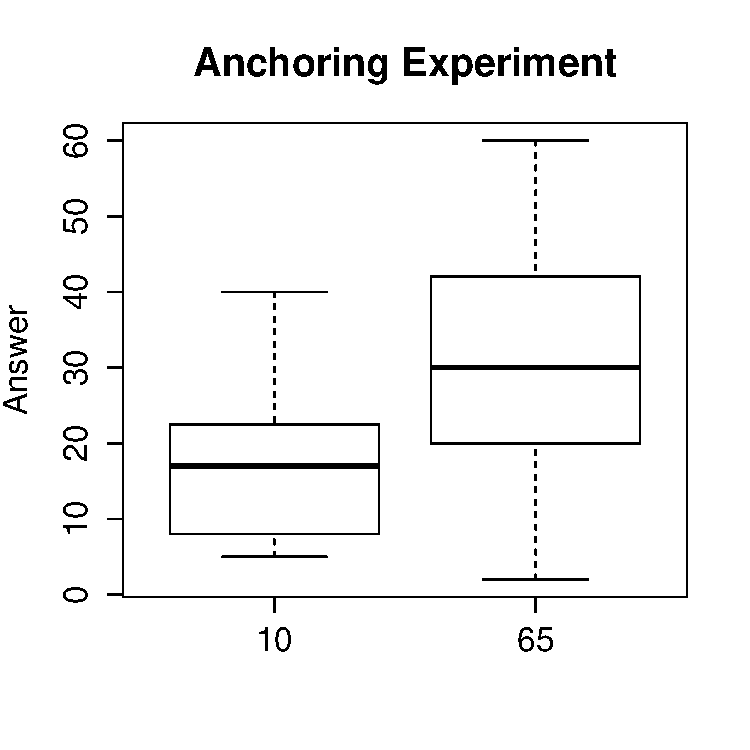
\includegraphics[scale = 0.4]{./images/anchoring_boxplot}
	\end{figure}

	\column{0.5\textwidth}
	\begin{block}{``Lo'' Group -- Shown 10 }
	$m_{Lo} = 43$\\ $\bar{y}_{Lo} = 17.1$ \\ $s^2_{Lo} = 86$
\end{block}
		\begin{block}{``Hi'' Group -- Shown 65 }
		$n_{Hi} =46$\\ $\bar{x}_{Hi} = 30.7$\\ $s^2_{Hi} = 253$
\end{block}

\end{columns}
\end{frame}
%%%%%%%%%%%%%%%%%%%%%%%%%%%%%%%%%%%%%%%%
\begin{frame}
\frametitle{ME for approx.\ 95\% for Difference of Means}

\small
\singlespacing
\begin{columns} 
	\column{0.5\textwidth}
	\begin{block}{``Lo'' Group}
		\begin{eqnarray*}
			\bar{y}_{Lo} &=&17.1 \\
			m_{Lo} &=& 43\\  
			s^2_{Lo} &=& 86\\ 
			\widehat{SE}(\bar{y}_{Lo})^2 &=& \frac{s^2_{Lo}}{m_{Lo}} = 2
		\end{eqnarray*}
	\end{block}
	
	\column{0.5\textwidth}
		\begin{block}{``Hi'' Group}
		\begin{eqnarray*}
			\bar{x}_{Hi} &=& 30.7\\
			n_{Hi} &=& 46\\  
			s^2_{Hi} &=& 253\\
			\widehat{SE}(\bar{x}_{Hi})^2 &=& \frac{s^2_{Hi}}{n_{Hi}} = 5.5
		\end{eqnarray*}
	\end{block}
\end{columns}

\pause
	\begin{eqnarray*}
		\bar{X}_{Hi} - \bar{Y}_{Lo} &=& 30.7 - 17.1 =  13.6\\ \pause
		\widehat{SE}(\bar{X}_{Hi} - \bar{Y}_{Lo}) &=& \pause \sqrt{\widehat{SE}(\bar{X}_{Hi})^2 + \widehat{SE}(\bar{Y}_{Lo})^2} = \sqrt{7.5}  \approx 2.7 \pause \Rightarrow ME \approx 5.4 \pause 
	\end{eqnarray*}
	$$\alert{\boxed{\mbox{Approximate 95\% CI} \quad (8.2, 19)}} \quad \mbox{What can we conclude?}$$


\end{frame}

%%%%%%%%%%%%%%%%%%%%%%%%%%%%%%%%%%%%%%%%
\section{CI for Difference of Population Proportions Using CLT}
%%%%%%%%%%%%%%%%%%%%%%%%%%%%%%%%%%%%%%%%
\begin{frame}
\frametitle{Confidence Interval for a Difference of Proportions via CLT}
	\begin{block}{What is the appropriate probability model for the sample?} 
$X_1, \hdots, X_n \sim \mbox{ iid Bernoulli}(p)$ independently  of $Y_1, \hdots, Y_m \sim \mbox{ iid Bernoulli}(q)$
\end{block}
	\begin{block}{What is the parameter of interest?}
The difference of population proportions $p - q$
\end{block}

\begin{block}{What is our estimator?}
The difference of sample proportions: $\widehat{p} - \widehat{q}$ where:
	$$\widehat{p} = \frac{1}{n}\sum_{i=1}^n X_i \quad \quad \quad	\widehat{q} = \frac{1}{m}\sum_{i=1}^m Y_i$$
\end{block}
\end{frame}

%%%%%%%%%%%%%%%%%%%%%%%%%%%%%%%%%%%%%%%%


\begin{frame}
\frametitle{Difference of Sample Proportions $\widehat{p}-\widehat{q}$ and the CLT}
\begin{block}{What We Have}
Approx.\ sampling dist.\ for \emph{individual} sample proportions from CLT:

\[\alert{\widehat{p} \approx N\left(p, \frac{\widehat{p}(1 - \widehat{p})}{n}\right), \quad \widehat{q} \approx N\left(q, \frac{\widehat{q}(1 - \widehat{q})}{m}\right)}\]
\end{block}

\begin{block}{What We Want}
Sampling Distribution of the \emph{difference} $\widehat{p} - \widehat{q}$
\end{block}

\begin{block}{Use Independence of the Two Samples}
  \[\alert{\widehat{p} - \widehat{q} \approx N\left( p - q, \frac{\widehat{p}(1 - \widehat{p})}{n} + \frac{\widehat{q} (1 - \widehat{q})}{m}\right)}\]
\end{block}

\end{frame}
%%%%%%%%%%%%%%%%%%%%%%%%%%%%%%%%%%%%%%%%
\begin{frame}

\frametitle{Approximate CI for Difference of Popn.\ Proportions $(p-q)$}


$X_1, \hdots, X_n \sim \mbox{iid Bernoulli}(p)$ \\
$Y_1, \hdots, Y_m \sim \mbox{iid Bernoulli}(q)$ \\
\emph{where each sample is independent of the other } 


  \[(\widehat{p} - \widehat{q}) \pm \texttt{qnorm}(1-\alpha/2)\; \widehat{SE}(\widehat{p} - \widehat{q})\] 

  \[
    \widehat{SE}(\widehat{p} - \widehat{q}) = \sqrt{\frac{\widehat{p}(1 - \widehat{p})}{n} + \frac{\widehat{q}(1 - \widehat{q})}{m}}
  \]


	\alert{Approximation based on the CLT. Works well provided $n,m$ large and $p,q$ aren't too close to zero or one.}

\end{frame}
%%%%%%%%%%%%%%%%%%%%%%%%%%%%%%%%%%%%%%%%
\begin{frame}
\frametitle{Are Republicans Better Informed Than Democrats?}
\framesubtitle{\fbox{\href{http://www.people-press.org/files/2012/08/8-10-12-Knowledge-release.pdf}{Pew: ``What Voters Know About Campaign 2012''}}}
Of the 239 Republicans surveyed, 47\% correctly identified John Roberts as the current chief justice. Only 31\% of the 238 Democrats surveyed correctly identified him. Is this difference meaningful or just sampling variation?

\vspace{2em}
\alert{Again, assume random sampling.}


\end{frame}
%%%%%%%%%%%%%%%%%%%%%%%%%%%%%%%%%%%%%%%%

\begin{frame}
\frametitle{ME for approx.\ 95\% for Difference of Proportions}

\footnotesize
\fbox{47\% of 239 Republicans vs.\ 31\% of 238 Democrats identified Roberts}
\singlespacing
\begin{columns} 
	\column{0.5\textwidth}
	\begin{block}{Republicans}
		\begin{eqnarray*}
			\widehat{p} &=& 0.47\\
			n &=& 239\\  \pause
			\widehat{SE}(\widehat{p}) &=&\sqrt{ \frac{\widehat{p}(1-\widehat{p})}{n}} \approx 0.032 \\ \pause
		\end{eqnarray*}
	\end{block}
	
	\column{0.5\textwidth}
		\begin{block}{Democrats}
		\begin{eqnarray*}
			\widehat{q} &=& 0.31\\
			m &=& 238\\  \pause
			\widehat{SE}(\widehat{q}) &=& \sqrt{\frac{\widehat{q}(1-\widehat{q})}{m}} \approx 0.030\\ \pause
		\end{eqnarray*}
	\end{block}
\end{columns}

\begin{block}{Difference: (Republicans - Democrats)}
	\begin{eqnarray*}
		\widehat{p} - \widehat{q} &=& 0.47 - 0.31 = 0.16\\ \pause
		\widehat{SE}(\widehat{p} - \widehat{q}) &=& \sqrt{\widehat{SE}(\widehat{p})^2 + \widehat{SE}(\widehat{q})^2} \approx 0.044  \pause \implies ME \approx 0.09 \pause 
	\end{eqnarray*}
	$$\alert{\boxed{\mbox{Approximate 95\% CI} \quad (0.07, 0.25)}} \quad \mbox{What can we conclude?}$$
\end{block}

\end{frame}
%%%%%%%%%%%%%%%%%%%%%%%%%%%%%%%%%%%%%%%%
\section{Matched Pairs versus Independent Samples}
%%%%%%%%%%%%%%%%%%%%%%%%%%%%%%%%%%%%%%%%

\begin{frame}
\frametitle{Which is the Harder Exam?}
Here are the scores from two midterms:
% latex.default(round(grades.out, 1), file = "grades.tex", rowname = NULL) 
%
\begin{table}[!tbp]
\begin{center}
\begin{tabular}{rrrr}
\hline\hline
\multicolumn{1}{r}{Student}&\multicolumn{1}{r}{Exam 1}&\multicolumn{1}{r}{Exam 2}&\multicolumn{1}{r}{Difference}\tabularnewline
\hline
$ 1$&$57.1$&$60.7$&$  3.6$\tabularnewline
$ 2$&$77.1$&$77.9$&$  0.7$\tabularnewline
$ 3$&$83.6$&$93.6$&$ 10.0$\tabularnewline
\vdots&\vdots&\vdots&\vdots\\
$69$&$75.0$&$74.3$&$ -0.7$\tabularnewline
$70$&$96.4$&$86.4$&$-10.0$\tabularnewline
$71$&$78.6$&$82.9$&$  4.3$\tabularnewline
\hline
Sample Mean: & 79.6 & 81.4  &1.8\\
\hline
\end{tabular}
\end{center}
\end{table}

\alert{Is it true that students score, on average, better on Exam 2 or is this just sampling variation?}
\end{frame}
%%%%%%%%%%%%%%%%%%%%%%%%%%%%%%%%%%%%%%%%
\begin{frame}
\frametitle{Are the two samples independent? \hfill 
\includegraphics[scale = 0.05]{./images/clicker}}
Suppose we treat the scores on the first midterm as one sample and the scores on the second as another. Are these samples independent?

\begin{enumerate}[(a)]
	\item Yes
	\item No
	\item Not Sure
\end{enumerate}


\end{frame}
%%%%%%%%%%%%%%%%%%%%%%%%%%%%%%%%%%%%%%%%
\begin{frame}
  \frametitle{Matched Pairs Data -- Dependent Samples}
The samples are dependent: each includes \alert{the same students}:
% latex.default(round(grades.out, 1), file = "grades.tex", rowname = NULL) 
%
\begin{table}[!tbp]
\begin{center}
\begin{tabular}{rccr}
\hline\hline
\multicolumn{1}{r}{Student}&\multicolumn{1}{c}{Exam 1}&\multicolumn{1}{c}{Exam 2}&\multicolumn{1}{r}{Difference}\tabularnewline
\hline
$ 1$&$57.1$&$60.7$&$  3.6$\tabularnewline
\vdots&\vdots&\vdots&\vdots\\
$71$&$78.6$&$82.9$&$  4.3$\tabularnewline
\hline
Sample Mean: & 79.6 & 81.4  &1.8\\
%Sample Var. &117  & 151 & 124\\
\alert{Sample Corr.} & \multicolumn{2}{c}{\alert{0.54}}&\\
\hline
\end{tabular}
\end{center}
\end{table}

This is really a \alert{one-sample} problem if we consider the \alert{difference} between each student's score on Exam 2 and Exam 1.
This setup is referred to as \alert{matched pairs data}.

\end{frame}
%%%%%%%%%%%%%%%%%%%%%%%%%%%%%%%%%%%%%%%%
\begin{frame}
\frametitle{Solving this as a One-Sample Problem}
\small
\fbox{Let $D_i = X_i - Y_i$ be the difference of student $i$'s exam scores.}

\vspace{2em}
I calculated the following in R:
	\begin{eqnarray*}
	\bar{D}_n &=& \frac{1}{n}\sum_{i=1}^n D_i \approx 1 .8\\
	S^2_D &=& \frac{1}{n-1}\sum_{i=1}^n (D_i - \bar{D})^2 \approx 	124\\ 
	\widehat{SE}(\bar{D}_n) &=&(S_D /\sqrt{n}) \approx \sqrt{124/71} \approx 1.3 
	\end{eqnarray*}
	
\vspace{1em}
\alert{Approximate 95\% CI Based on the CLT:}
$$\alert{\boxed{1.8 \pm 2.6 = (-0.8, 4.4)}} \quad \mbox{What is our conclusion?}$$

\end{frame}
%%%%%%%%%%%%%%%%%%%%%%%%%%%%%%%%%%%%%%%%
\begin{frame}
	\begin{center}
	\Huge How are the Independent Samples and Matched Pairs Problems Related?
	\end{center}
\end{frame}

%%%%%%%%%%%%%%%%%%%%%%%%%%%%%%%%%%%%%%%%
\begin{frame}
\frametitle{Difference of Means = Mean of Differences?\hfill 
\includegraphics[scale = 0.05]{./images/clicker}}
\fbox{Let $D_i = X_i - Y_i$ be the difference of student $i$'s exam scores.}

True or False:
	$$\bar{D}_n = \bar{X}_n - \bar{Y}_n$$

\begin{enumerate}[(a)]
	\item True
	\item False
	\item Not Sure
\end{enumerate}

\end{frame}
%%%%%%%%%%%%%%%%%%%%%%%%%%%%%%%%%%%%%%%%
\begin{frame}
\frametitle{Difference of Means Equals Mean of Differences}

\small

\begin{eqnarray*}
	\bar{D}_n &=& \frac{1}{n}\sum_{i=1}^n D_i = \frac{1}{n}\sum_{i=1}^n (X_i - Y_i) = \bar{X}_n - \bar{Y}_n
\end{eqnarray*}

% latex.default(round(grades.out, 1), file = "grades.tex", rowname = NULL) 
%
\begin{table}[!tbp]
\begin{center}
\begin{tabular}{rccr}
\hline\hline
\multicolumn{1}{r}{Student}&\multicolumn{1}{c}{Exam 1}&\multicolumn{1}{c}{Exam 2}&\multicolumn{1}{r}{Difference}\tabularnewline
\hline
$ 1$&$57.1$&$60.7$&$  3.6$\tabularnewline
\vdots&\vdots&\vdots&\vdots\\
$71$&$78.6$&$82.9$&$  4.3$\tabularnewline
\hline
Sample Mean: & 79.6 & 81.4  &1.8\\
\hline
\end{tabular}
\end{center}
\end{table}


\begin{eqnarray*}
	\bar{D}_n &=& 1.8\\ 
	\bar{X}_n - \bar{Y}_n &=&  81.4 - 79.6 =   1.8  \;\alert{\checkmark}
\end{eqnarray*}

\end{frame}

%%%%%%%%%%%%%%%%%%%%%%%%%%%%%%%%%%%%%%%%

\begin{frame}
\frametitle{...But Correlation Affects the Variance}
\footnotesize
\begin{eqnarray*}
	S_D^2&=& \frac{1}{n-1}\sum_{i=1}^n \left( D_i - \bar{D}_n\right)^2 = \pause \frac{1}{n-1}\sum_{i=1}^n \left[ \left( X_i - Y_i\right) - \left( \bar{X}_n - \bar{Y}_n\right)\right]^2\\ \pause
	&=&\frac{1}{n-1}\sum_{i=1}^n \left[ \left( X_i - \bar{X}_n\right) - \left( Y_i - \bar{Y}_n\right)\right]^2\\ \pause
	&=&\frac{1}{n-1}\sum_{i=1}^n \left[ \left( X_i - \bar{X}_n\right)^2 + \left( Y_i - \bar{Y}_n\right)^2 - 2\left(X_i - \bar{X}_n\right)\left(Y_i - \bar{Y}_n\right)\right]\\ \pause
	&=& S_X^2 + S_Y^2 - 2 S_{XY}\\ \pause
	&=& S_X^2 + S_Y^2 - 2 S_X S_Y r_{XY}
\end{eqnarray*}

\pause

\vspace{1em}
\alert{$\boxed{r_{XY} > 0 \implies S_D^2 < S_X^2 + S_Y^2}$} \\ \pause
\alert{$\boxed{r_{XY} = 0 \implies S_D^2 = S_X^2 + S_Y^2}$} \\ \pause
\alert{$\boxed{r_{XY} < 0 \implies S_D^2 > S_X^2 + S_Y^2}$}

\end{frame}
%%%%%%%%%%%%%%%%%%%%%%%%%%%%%%%%%%%%%%%%
\begin{frame}
\frametitle{Dependent Samples -- Calculating the ME}
% latex.default(round(grades.out, 1), file = "grades.tex", rowname = NULL) 
%
\begin{table}[!tbp]
\begin{center}
\begin{tabular}{rccr}
\hline\hline
\multicolumn{1}{r}{Student}&\multicolumn{1}{c}{Exam 1}&\multicolumn{1}{c}{Exam 2}&\multicolumn{1}{r}{Difference}\tabularnewline
\hline
$ 1$&$57.1$&$60.7$&$  3.6$\tabularnewline
\vdots&\vdots&\vdots&\vdots\\
$71$&$78.6$&$82.9$&$  4.3$\tabularnewline
\hline
Sample Var. &117  & 151 & \alert{\fbox{?}}\\
Sample Corr.& \multicolumn{2}{c}{0.54}&\\
\hline
\end{tabular}
\end{center}
\end{table}

$$117 + 151 - 2 \times 0.54 \times \sqrt{117 \times 151} \approx 124   \;\alert{\checkmark}$$

\alert{This agrees with our calculations based on the differences.}
\end{frame}
%%%%%%%%%%%%%%%%%%%%%%%%%%%%%%%%%%%%%%%%
\begin{frame}
\frametitle{The ``Wrong CI'' (Assuming Independence)}
\footnotesize
% latex.default(round(grades.out, 1), file = "grades.tex", rowname = NULL) 
%
\begin{table}[!tbp]
\begin{center}
\begin{tabular}{rccr}
\hline\hline
\multicolumn{1}{r}{Student}&\multicolumn{1}{c}{Exam 1}&\multicolumn{1}{c}{Exam 2}&\multicolumn{1}{r}{Difference}\tabularnewline
\hline
Sample Size & 71 & 71 & 71\\
Sample Mean & 79.6 & 81.4  &1.8\\
Sample Var. &117  & 151 & 124\\
Sample Corr.& \multicolumn{2}{c}{0.54}&\\
\hline
\end{tabular}
\end{center}
\end{table}

\singlespacing
\small

\begin{block}{Wrong Interval -- Assumes Independence}
$$1.8 \pm 2\times  \sqrt{117/71 + 151/71} \implies (-2.1, 5.7)$$
\end{block}

\pause

\begin{block}{Correct Interval -- Matched Pairs}
$$1.8 \pm 2\times  \sqrt{124/71} \implies (-0.8, 4.4)$$
\end{block}

\pause
\alert{Top CI is too wide: since exam scores are positively correlated the variance of the differences is less than the sum of the variances.} 

\end{frame}
%%%%%%%%%%%%%%%%%%%%%%%%%%%%%%%%%%%%%%%%


\begin{frame}
\frametitle{CIs for a Difference of Means -- Two Cases}

\begin{block}{Independent Samples}
 Two independent samples: $X_1, \dots, X_n$ and $Y_1, \dots, Y_m$. 
\end{block}

\begin{block}{Matched Pairs}
 Matched pairs $(X_1, Y_1), \dots, (X_n, Y_n)$ where $X_i$ is \alert{not independent} of $Y_i$ but each pair $(X_i, Y_i)$ is independent of the other pairs. 
\end{block}

\begin{alertblock}{Crucial Points}
\begin{itemize}
	\item Learn to recognize matched pairs and independent samples setups since the CIs are different! 
	\item Two equivalent ways to construct matched pairs CI:
		\begin{enumerate}
			\item Method 1: use sample mean and std.\ dev.\ of $D_i = X_i - Y_i$ 
      \item Method 2: use $\bar{X}_n$, $\bar{Y}_n$, along with $S_X$, $S_Y$ and $r_{XY}$
		\end{enumerate}
\end{itemize}
\end{alertblock}

\end{frame}
%%%%%%%%%%%%%%%%%%%%%%%%%%%%%%%%%%%%%%%%

